\section{Continuous Integration}
Projektet er sat op, så der blev benyttet continuous integration. Dette betød, at projektet bliver bygget på en ekstern server, hver gang der bliver tilføjet en ændring til projektet via git. CI er blevet brugt for at undgå integrationsproblemer i projektet. Disse kan nemt opstå, når flere personer arbejder parallelt på projektet. CI har ved at bygge projektet hele tiden holdt styr på projektets status. Så hvis der opstod problemer på projektet kunne de nemt lokaliseres til et enkelt push. Dette har været med til at overskueliggøre processen for alle gruppemedlemmer.
TeamCity blev sat op med to build som var afhængige af hinanden. Efter hvert push til repositoriet blev projektet bygget. Hvis projektet kunne bygges blev 
\\
\noindent TeamCity blev anvendt som CI-server, hvor der blev opsat et  projekt, der blev sat til at pege på gruppens github-repository. Projektet blev sat op til, at hver gang der blev "pushed" til reopistoriet skulle TeamCity kører to "Build Steps". I første step blev projektet bygget ved brug af MSBuild Tools 2015. Hvis det første skridt gik godt blev anden step udført, der bestod i at køre Test-projektets NUnit-tests. Testene blev kørt ved brug af en NUnit.ConsoleRunner, der var blevet installeret som en NuGet-Package i projektet.  
CI-projeket blev også tilknyttet en dotCover-test, der skulle fungere som et pejlemærke for, hvor stor en del af projektet testene dækker. Da der ikke var nogen specielle krav til Coverage-analysen blev JetBrains standard dotCover fil benyttet.

\noindent Nedenunder på figur \ref{fig:TeamCityTest} kan et eksempel af et build på TeamCity serveren ses. 
\begin{figure}[ht!]
	\centering
	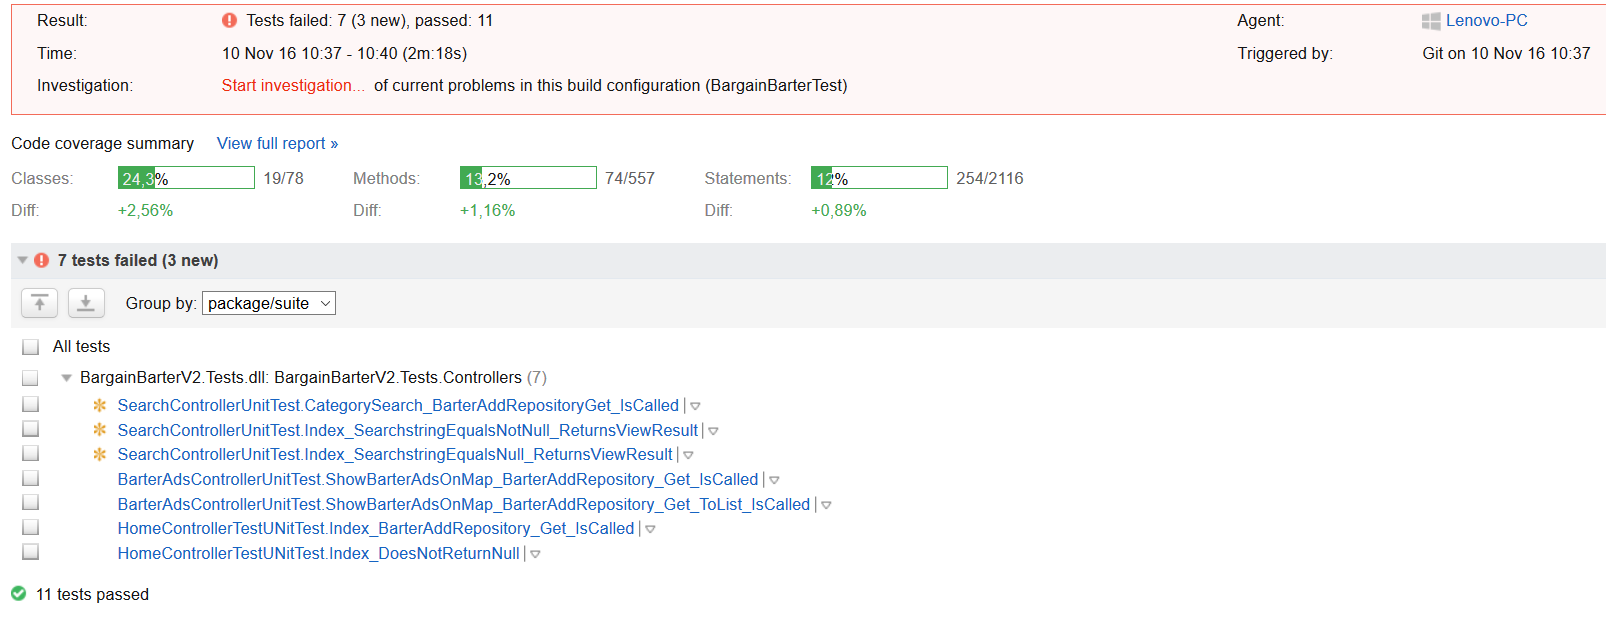
\includegraphics[width=120mm]{figures/TeamCityTest.png}
	\caption{Testresultat på baggrund af kørte test på TeamCity}
	\label{fig:TeamCityTest}
\end{figure}
\\
Som det fremgår af figur \ref{fig:TeamCityTest} gav TeamCity et let og overskueligt overblik og projektets status, der kunne blandt andet ses Coverage-analysen og hvilke test, der fejlede mm.
\\
Det var et bevidst valg fra gruppens side at benytte TeamCity i stedet for Jenkins, der er opnået erfaring med i undervisningen i I4SWT, for at opnå erfaring med forskellige CI-servere og programmer.